\section{Evaluación empírica}

Para evaluar el rendimeinto, se ha usado el \textit{script} de Python \href{run:./src/test.py}{\texttt{src/test.py}}.\\
Se ha ejecutado cada función en todo el rango de valores posibles que permite el sistema, desde números un dígito, hasta lo máximo posible, en este caso números de 20 digitos. Para obtener dicho número máximo, se emplean la variables \texttt{primeslib.MAX\_UINT} y \texttt{gcdlib.MAX\_INT} que retonan el mayor número posible de computar para cada librería.\\
\\
Para cada longitud de numeros se calculan un total de 400 numeros aleatorios y se aplica la función a cada uno de ellos para determinar si son primos. Así se obtiene la media de tiempo de ejecución para dicha longitud de número, buscando obtener resultados lo más fiables posible, evitando así que los casos extremos distorsionen dichos resultados.\\

Una vez obtenidos los resultado indicados previamente, se guardan en formato CSV en la carpeta \texttt{data/} y se representan gráficamente mediante la librería \href{https://matplotlib.org/}{matplotlib}.

\subsection{Test de primalidad}
Se comprueba como el tiempo de ejecución se mantiene estable con pequeñas variaciones para números de hasta 15 digitos, de ahí en adelante se aprecia que cada aumento de tamaño de número se traduce en un aumento cada vez más significativo en el tiempo de ejecución.\\
\\
Pese a que el grafico muestre una distribución de resultados logarítmica, esto se debe a que la escala muestra en el eje x el numero de digitos de los números, por lo tanto la escala no avanza de manera lineal ya que por cada digito que aumenta, la cantidad de números aumenta en mayor medida que para el número de digtos previo. Es por ello, que pese a que se muestre una distribución logarítmica, si la escala empleada para mostrar el gráfico fuese lineal se mostraría el grafico de manera lineal. A continuación se incluye dicho grafico:

\begin{figure}[H]
	\makebox[\textwidth][c]{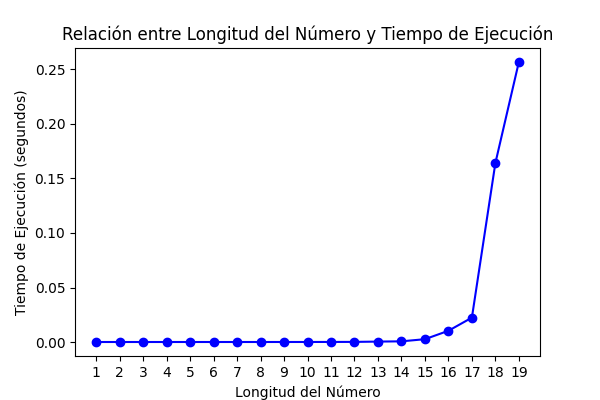
\includegraphics[width=15cm]{img/scatter_plot_primes.png}}
\end{figure}

Una vez obtenidos los resultados empíricos, para poder comparar si dichos resultados obtenidos son correctos se obtiene el graico generado a aprtir de aplicar la función teórica, al igual que en la obtención de resultados previos, a numeros de distinta longitud de dígitos. Pese a que las magnitudes de tiempo meidas no son identicas, porporcionalmente se observa que ambos gráficossiguen tendencias muy similares, por lo que se interpreta que los resultados obtenidos son correctos.

\begin{figure}[H]
	\makebox[\textwidth][c]{\includegraphics[width=15cm]{img/scatter_plot_primes_theoretical.png}}
\end{figure}

También se incluye el gráfico recogiendo los tiempos de ejecución únicamente para los números primos, donde se observa que la tendencia cambia mostrando un incremento de tiempo de ejecución más pronunciado desde el comienzo.
\begin{figure}[H]
	\makebox[\textwidth][c]{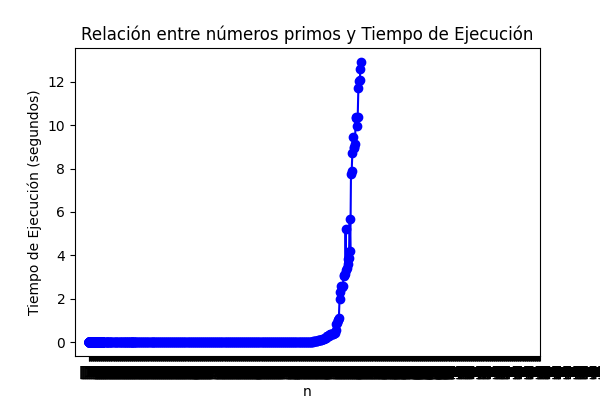
\includegraphics[width=15cm]{img/scatter_plot_primes_only_primes.png}}
\end{figure}

Por último se muestra el gráfico generado a aprtir de los resultados obtenidos con casos extremos que requieren tiempos de ejecución mayores a la media, dichos números se han obtenido del listado proporcionado en aulaglobal
\begin{figure}[H]
	\makebox[\textwidth][c]{\includegraphics[width=15cm]{img/scatter_plot_primes_worst_cases.png}}
\end{figure}




\subsection{Cálculo de Máximo Común Divisor}

\subsubsection{Descomposición en factores primos}
Para este caso, debido al tiempo de ejecución, para esta prueba redujimos el número de iteraciones a 5 y el máximo de dígitos a 11, ya que no a partir de dicho número de dígitos no resultaba viable la ejecución debido, al tiempo que esta requería- Pese a reducir la cantidad de números, se observa una tendencia clara, en como con cada aumento de dígitos aumenta considerablemente 
\begin{figure}[H]
	\makebox[\textwidth][c]{\includegraphics[width=15cm]{img/scatter_plot_gcd_factorize.png}}
\end{figure}

Una vez obtenidos los resultados empíricos, se genera el gráfico a parir de la función teórica con el fin de comprobar si los resultados obtenidos son correctos. Efectivamnete se observa como la tendencia en ambos gráficos es muy similar por lo que se puede inferir que los resultados son lo esperado. Puesto que como ya se mencionó previamnete pese a que se muestre una distribución logarítmica, se debe a que el ejer X pese a estar representado de manera lineal la distancai entre dígitos, esta debería ser cada vez mayor puesto que a más digitos más numeros posibles. Es por ello que si se siguese un eje X como el descrito la distribución se mostraría lineal
\begin{figure}[H]
	\makebox[\textwidth][c]{\includegraphics[width=15cm]{img/scatter_plot_gcd_theoretical_factorize.png}}
\end{figure}



\subsubsection{Método de Euclides}
Por último se han realizado las pruebas empíricas con el alrgoritmo de Ecuclides para calcular el máximo común divisor, donde so observan resultados duisparos auqnue una moderada tendencia de incremneto de teimo en función del número de dígitos
\begin{figure}[H]
	\makebox[\textwidth][c]{\includegraphics[width=15cm]{img/scatter_plot_gcd_euclid.png}}
\end{figure}

A su vez se ha obtenido también el gráfico generado a partir de emplear la función teórica
\begin{figure}[H]
	\makebox[\textwidth][c]{\includegraphics[width=15cm]{img/scatter_plot_gcd_theoretical_euclid.png}}
\end{figure}